\renewcommand{\thechapter}{7}

\chapter{The electron recoil band of LUX}
\label{Ch:T}

In this chapter we overview the development, implementation and the main results of the tritiated-methane calibration source. The source was developed to be a method of calibrating the electronic recoil (ER) band in current and future large scale xenon detectors (+100 kg). As opposed to external ER calibration sources, the tritiated-methane is internal and mixes with the bulk xenon. Internal sources have a great advantage over external sources as they trivially overcome the formidable stopping power of liquid xenon, illuminating the fiducial volume of the detector. The tritiated-methane calibration source was ultimately used to characterize background ER events in LUX. Once the ER band is defined the background rejection of WIMP candidates at a particular energy is treated with a profile likelihood analysis, described in \cite{LUX_PRL}.

\section{The need for an Internal Calibration Source} %Tritiated-Methane as a Calibration Source

Over the past two decades liquid nobel TPCs used for dark-matter experiments have grown to net more kg-days of exposure. With the additional mass, nobel detectors benefit from the self shielding properties of the dense liquid inside the inner fiducial volume of the detector, as the outer volume is used as an active veto \cite{Aprile_LXe_overview}. With current generation liquid xenon detectors containing more than 100 kg, the detectors are virtually insensitive to external gamma radiation in the WIMP search region of interest of 1-10 $\rm keV_{ee}$ \cite{LUX_BG} \cite{Xenon100} \cite{PandaX} \cite{XMass}. Being insensitive to external radioactivity improves the signal to background ratio for WIMP searches. Unfortunately, it is also shields against external calibration sources. With plans for even larger xenon detectors already moving forward \cite{LZ} \cite{Xenon1T}, we must develop a new method for introducing controlled radioactivity for calibration purposes.

The fiducial volume of the LUX detector is surrounded by more than than 6 cm of liquid xenon providing excellent shielding from both external backgrounds and calibration sources \cite{LUX_BG}. For example, a 100 keV gamma has a mean free path of about 2 mm in liquid xenon and would require thirty mean free paths to penetrate into the fiducial volume. A higher energy source such as $\rm ^{137}Cs$ (662 keV) has a longer mean free path of 4 cm however, the probability of a low energy deposit from forward scattering in the fiducial followed by an escape is greatly suppressed. We would expect less than one ER event per day between 1-10 $\rm keV_{ee}$ in the fiducial region if calibrating with an external $\rm ^{137}Cs$ or Th source, \cite{LUX_BG}. Furthermore, calibrating with high energy sources or high rate sources introduces systematic uncertainties from high energy deposits near the detector edge, the high rates would also overwhelm the DAQ.  

\section{Tritiated-Methane as a Calibration Source}
To overcome the issues with external calibrations, the source used to calibrate the ER band must satisfy three requirements. First, it should illuminate the WIMP search band with single scatter events (1-10 $\rm keV_{ee}$). Second, it must be able to mix with the xenon and be delivered as an internal source. Third, it should either have a short half-life or be easily separated from xenon by commercially available gettering technology. \KrCal has been developed and used as an internal source with liquid xenon detectors \cite{Kastens} \cite{Baudis}. However, in LUX \KrCal only produces a mono-energetic peak at 42.1 $\rm keV_{ee}$, which is too high in energy to calibrate the WIMP search region. In order to populate the ER band with single scatter events between 1- 10 keV a beta emitter should be injected. Tritium is an ideal candidate, satisfying all but the removal requirement. Tritium has a Q value of 18.6 keV \cite{Tritium_Q}, a mean beta energy of 5.6 keV \cite{Tritium_Mean} and a mode of 3 keV \cite{Tritium_Eq}, (see figure \ref{fig:True_T_Spec}).


\begin{figure}[h!]\centering
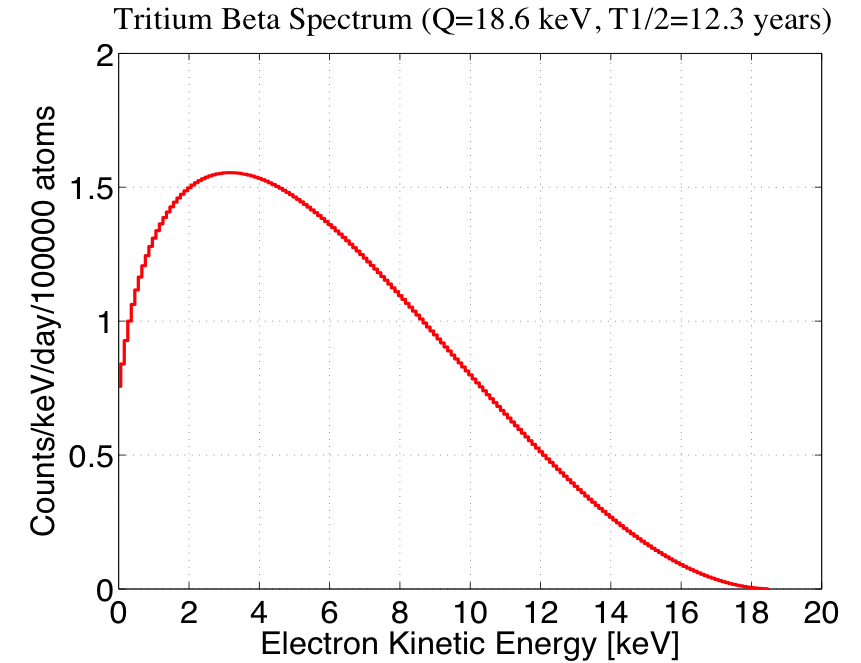
\includegraphics[width=120mm]{Tritium_Source/Tritium_Spectrum.png}
\caption{True tritium beta spectrum from \cite{Tritium_Eq}. }
\label{fig:True_T_Spec}
\end{figure}


Tritium has a half life of 12.3 years \cite{Tritium_halflife_all}. Thus, it is not practical to wait for the tritium activity to decay away. The tritium must be removed after the calibration is complete in order to continue a low background WIMP search run. Hydrogen, being chemically identical to tritium, can be removed from the bulk xenon by standard gettering technology \cite{SAES}. However, the removal is complicated by tritium's high diffusion rate into plastics and other detector materials \cite{miyake:1983}. Failure to remove the tritium would mark the end of a dark matter search. 

To mitigate the effect of tritium diffusion into plastics we use a tritiated-methane source instead of bare tritium. Tritiated-methane consists of a tritium atom and three hydrogen atoms bound to a carbon molecule, and is chemically identical to methane. Using tritiated-methane reduces the diffusion of tritium into detector internals by an order of magnitude \cite{miyake:1983}. The weak molecular bond,  $<$ 1 eV, to the methane molecule does not impact the nuclear physics of the tritium beta decay. Also, methane is known to be soluble in liquid xenon and is sometimes used to quench scintillation light when injected in relatively large amounts \cite{bondar2006two}, \cite{Kirill_Methane}, \cite{Shibamura}. Finally, we have studied the removal of methane by the SAES heated zirconium getter (used in LUX) and found that significant amounts of methane can be removed from xenon at our flow rates \cite{Dobi_CH4},\cite{coldtrap}. 


\section{Removal of $\rm CH_4$ from LUX}

The injection and removal of tritiated-methane into a liquid xenon vessel containing plastics was first conducted in an experimental setup at UMD. Even with conservative estimates for diffusion rates into plastics, we could not be certain about the behavior of tritiated-methane in the much larger LUX detector. Prior to injecting the tritiated-methane into LUX a much larger natural methane (non-tritiated) injection was performed in order to characterize diffusion, being chemically identical tritiated-methane. A xenon gas analysis system, developed at the University of Maryland, allowed for on site purity analysis from several ports plumbed directly into the LUX xenon circulation loop. The analysis system has ppt (part-per-trillion) sensitivity to $\rm CH_4$ and better than ppt sensitivity to $\rm Kr$. The compact system allows for hourly sampling and is used for detection of several key impurities ($\rm N_2$, $\rm O_2$, $\rm He$, $\rm Ar$, $\rm Kr$, $\rm CH_4$, $\rm H_2$). The system is  significantly less expensive than the more complex techniques used by \cite{ATTA} and \cite{Kr_ppq}. The purity analysis technique is described in \cite{coldtrap}, \cite{Dobi_CH4}, \cite{EXO_SAM}, \cite{Kr_ppt_Dobi},  and will be described specifically for the LUX system in a future publication. %The development of the tritiated-methane calibration source will be described in a future publication [Tritium Paper Place Holder].

Figure \ref{fig:Removal_Methane} shows the results from the xenon gas analysis system for a 50 ppb (g/g) methane injection into the bulk xenon. The xenon of the LUX detector is continually cycled at 27 SLPM, with the xenon gas being passed through a heated zirconium getter which removes impurities, including methane. After the first hour, the 50 ppb of methane mixes into the liquid and appears as 300 ppb in the gas returning from the bulk liquid. The enhancement in the gas phase is due to the solubility of methane dissolved in liquid xenon and is characterized by the Henry's constant .

\renewcommand{\baselinestretch}{1}
\small\normalsize
\begin{figure}[h!]\centering
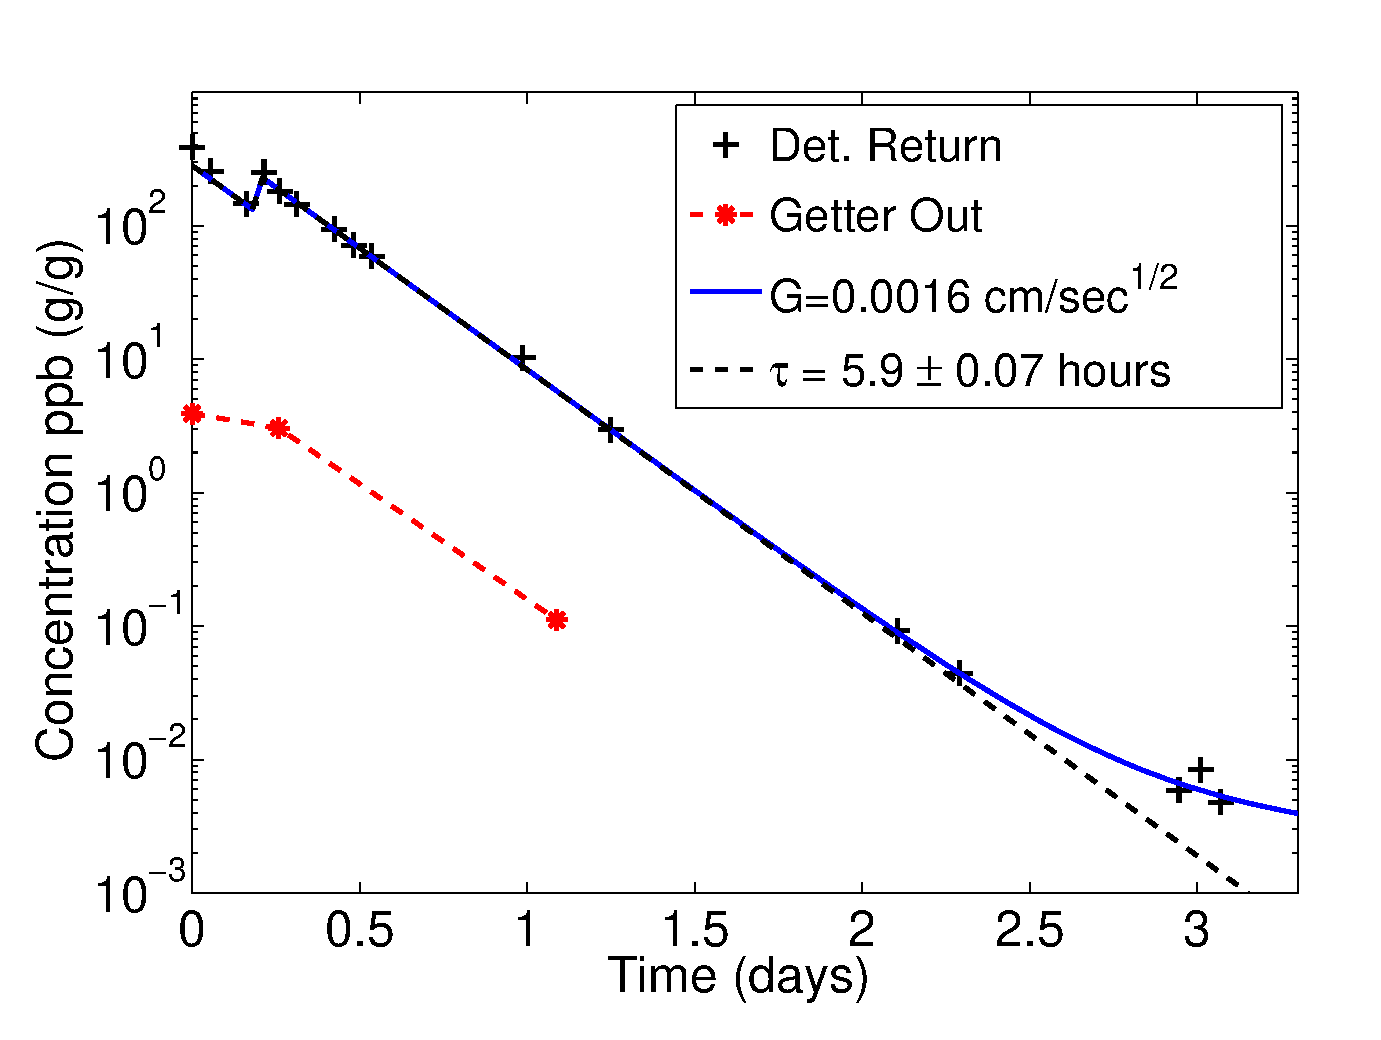
\includegraphics[width=120mm]{Chapter_T/Figures/July_CH4_wOG.eps}
\caption{Removal of natural methane observed by the integrated xenon sampling system prior to the tritiated-methane injections. The red points indicate measurements at the getter outlet. We find a 97\% one-pass removal efficiency at a flow rate of 27 SLPM. The blue curve shows the improved upper limit on the effect of outgassing from the plastics. The black dashed lines shows the exponential fit to the natural methane removal from the xenon with a time constant of 5.9 $\pm 0.07$ hours. $\rm 5\times10^{-3}$ ppb (g/g) is the limit of detection for methane.}
\label{fig:Removal_Methane}
\end{figure}
\renewcommand{\baselinestretch}{2}
\small\normalsize

The measurements provided crucial diagnostics for methane removal and diffusion into plastic components in the LUX detector. We measured the one-pass purification efficiency for methane to be 97\% by the SAES PS4-MT15-R-1 MonoTorr getter (\cite{SAES}) at a xenon gas flow rate of 27 SLPM. The getter's health for hydrocarbon removal is important to check prior to a tritiated methane injection, as an aged zirconium getter will lose its ability to remove $\rm CH_4$ before failing for $\rm N_2$ and $\rm O_2$ \cite{Dobi_CH4}. We confirmed that natural methane could be removed by more than five orders of magnitude without residual back diffusion. (The plateau seen in the end of figure \ref{fig:Removal_Methane} is caused by the 5 ppt limit for methane detection rather than diffusion from plastic components which absorb the impurity when it is initially injected). %Taking the background as the limit for back diffusion we infer a diffusion constant of less than 1.6$\rm \times 10^{-3} \, cm/sec^{1/2} $. 

The results from the natural methane injection gave us the confidence to proceed with injecting tritiated methane, knowing that the goal of reducing the tritium rate to less than 5\% of background could be met in the LUX detector. The purification time constant for natural methane removal was measured to be $\rm 5.9 \pm 0.07$ hours as seen in figure \ref{fig:Removal_Methane}. The removal time constant is $\rm 1/6$ of that expected based on xenon circulation rates alone, and is exactly the ratio of methane concentration in the gas to the methane concentration in the liquid. The enhanced purification time constant is reasonable as the methane is purified from the gas phase where it is more abundant, with the equilibrium concentration in the gas above the liquid set by the solubility.

%Having an integrated xenon gas sampling system, developed for LUX to monitor krypton daily \cite{Kr_ppt_Dobi} \cite{EXO_SAM}, allowed us to conduct situ methane measurements providing a diagnostic of the natural methane diffusion without the risk of permanent tritium contamination. Before injecting tritiated-methane into the detector we first injected $\rm 1/10^{6}$ (g/g) of natural methane and demonstrated its removal from the LUX xenon to five orders of magnitude, this allowed us to proceed with confidence knowing that the goal of reducing the tritium rate to less than 5\% of background could be met. Methane is chemically identical to tritiated-methane and having the ability to sample the gas proved useful for the tritium campaign, the purification time constant for natural methane removal was measured to be $\rm 5.9 \pm 0.07$ hours with the xenon gas sampling system \ref{fig:Removal_methane}. The removal time constant was $\rm 1/5$ of that expected based on xenon circulation rates alone, potentially enhanced by the solubility of methane between the liquid and gaseous xenon. The enhanced purification time constant allowed for larger injections of tritiated-methane into the detector. 


\section{Light Yield Quenching from $\rm CH_4$ in LUX}

It is well known that at high concentrations (several percent) methane will quench scintillation in liquid xenon \cite{bondar2006two}, \cite{Kirill_Methane}, \cite{Shibamura} \cite{Xe_CH4_Theory}. The quenching of scintillation in liquid argon has been observed with methane concentrations as low as 10 ppb (part-per-billion) \cite{Ar_CH4}. When performing a tritiated-methane calibration for the LUX detector, containing 350 kg of xenon, the amount of natural methane injected is $<$10 ppt (parts-per-trillion). This is far too low to cause any shift in the observed light yield and impact the ER band measurement. To prove this, a natural methane injection of 1 ppm (parts per million) was performed along with periodic \KrCal calibrations that were used to track the light yield of the line source normalized at the center of the detector. Figure \ref{fig:Methane_LY} shows the result of \KrCal calibration along with the methane concentration in the gas measured by the analysis system.

\renewcommand{\baselinestretch}{1}
\small\normalsize
\begin{figure}[h!]\centering
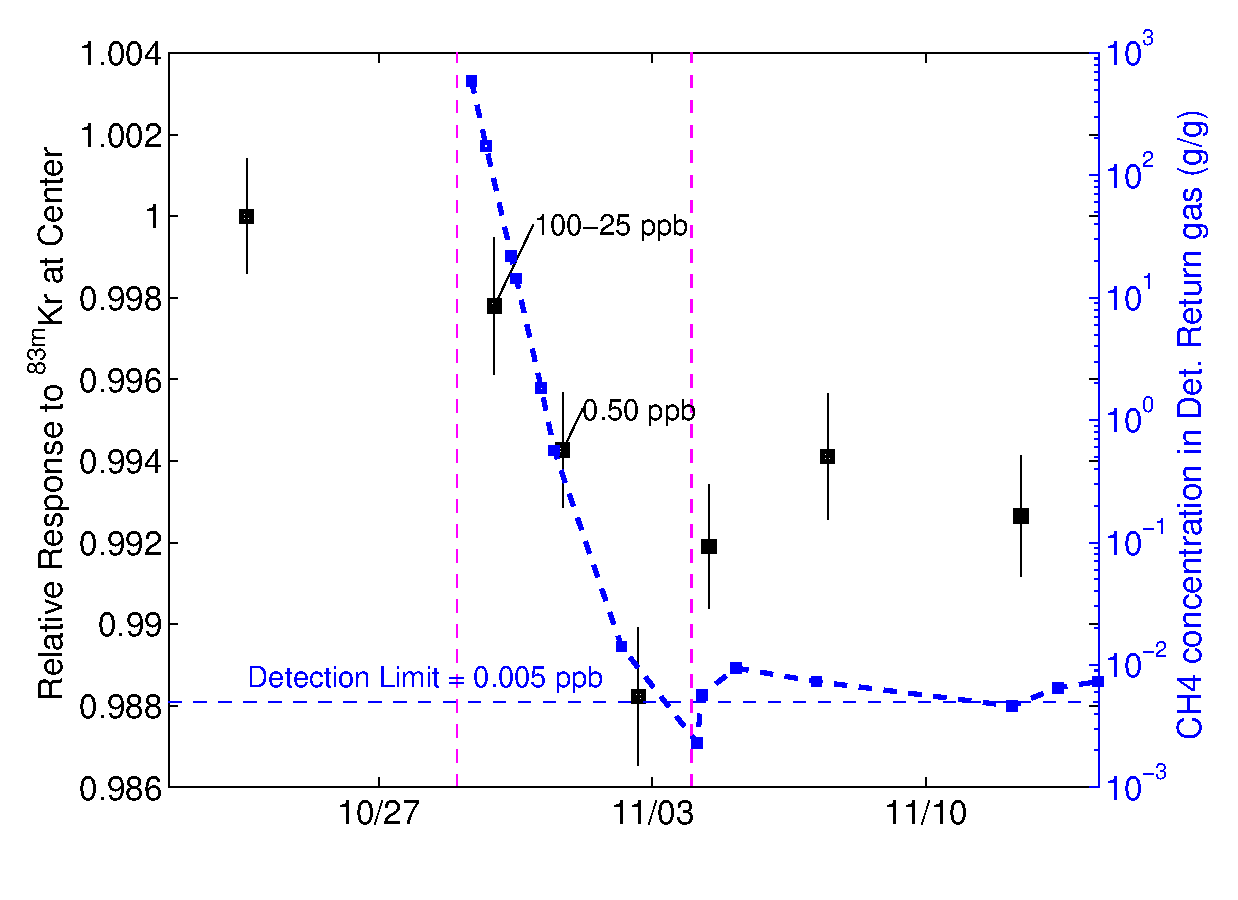
\includegraphics[width=120mm]{Chapter_T/Figures/CH4/CH4_Kr.eps}
\caption{In black, the response to scintillation from \KrCal at the center of the detector normalized to the first data point before the natural methane ($\rm CH_4$) injection. The dashed magenta lines represent the time window from the beginning of the natural methane injection to the time the background of 5 ppt is reached. The blue points represent that methane concentration in the gas returning from the bulk liquid of the detector. The concentration in the liquid xenon is roughly 1/6 of the concentration measured in the gas phase due to solubility.  }
\label{fig:Methane_LY}
\end{figure}
\renewcommand{\baselinestretch}{2}
\small\normalsize

In figure \ref{fig:Methane_LY}, there are two \KrCal data sets that had methane concentrations above background levels. The first measurement is made with greater than 25 ppb in the gas corresponding to greater than 4 ppb in the liquid. The second contained greater than 500 ppt in the gas corresponding to greater than 83 ppt in the liquid. The shifts in yield are purely systematic, as the two light yield measurements containing methane fall between the measured yields of the first (prior to injection) and last (well below 5ppt) data points. We constrain light yield quenching induced by 4 ppb (g/g) of methane in liquid xenon to $<1\%$. Note, that a typical tritiated-methane calibration contains roughly three orders of magnitude less methane than 4 ppb (g/g).


\subsection{Tritiated Methane injection into the LUX detector}

Following the natural methane test, the tritiated-methane injection was conducted at the end of the first underground science run, on Aug 8th 2013. An absolute activity of 20 mBq of tritiated-methane was injected at the purifier's outlet while circulating the xenon at 27 SLPM. A removal time constant of $\rm 6.0 \pm 0.5$ hours was measured in the liquid volume (figure \ref{fig:Removal}) and is consistent with the natural methane removal measured in the gas by the sampling system (figure \ref{fig:Removal_Methane}). 

After a day of circulating through the getter the tritium decay rate had fallen below detectable levels confirming the effective removal of the tritiated-methane with the getter. A second, larger injection of 800 mBq was performed a week later yielding a similar removal time constant of $\rm 6.4 \pm 0.1$. The second injection produced 20,000 beta decays in the LUX detector, 7000 of which were in the fiducial volume and could be used to calibrate the ER band in the WIMP search region of 1-50 PE (about 1-8 $\rm keV{ee}$). Prior to LUX detector upgrades in December 2013, a total of 10 Bq of tritiated-methane was injected into the LUX detector and successfully removed providing over 140,000 beta decays within the fiducial volume. 

\renewcommand{\baselinestretch}{1}
\small\normalsize
\begin{figure}[h!]\centering
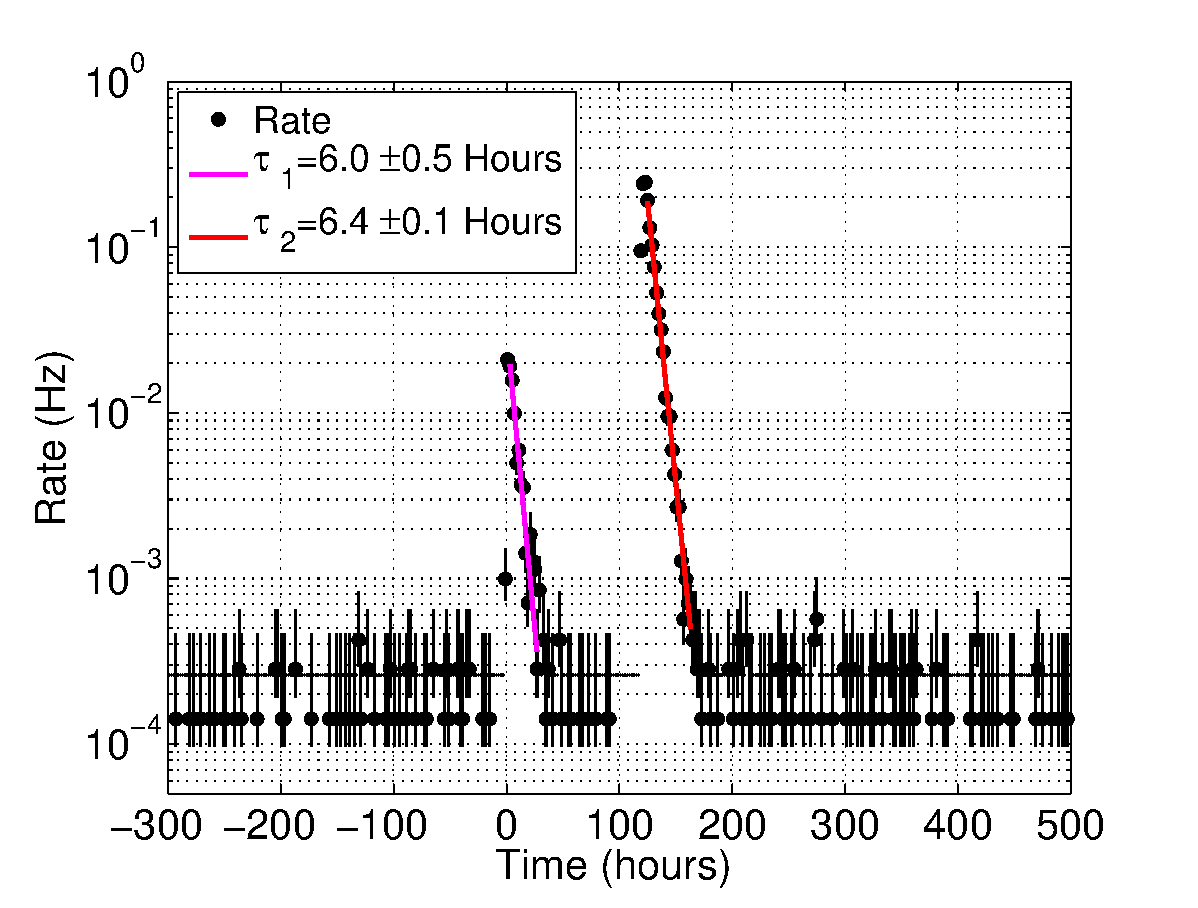
\includegraphics[width=120mm]{Chapter_T/Figures/CH3T_Rate_fid_150_Run03_Tritium_Rate.eps}
%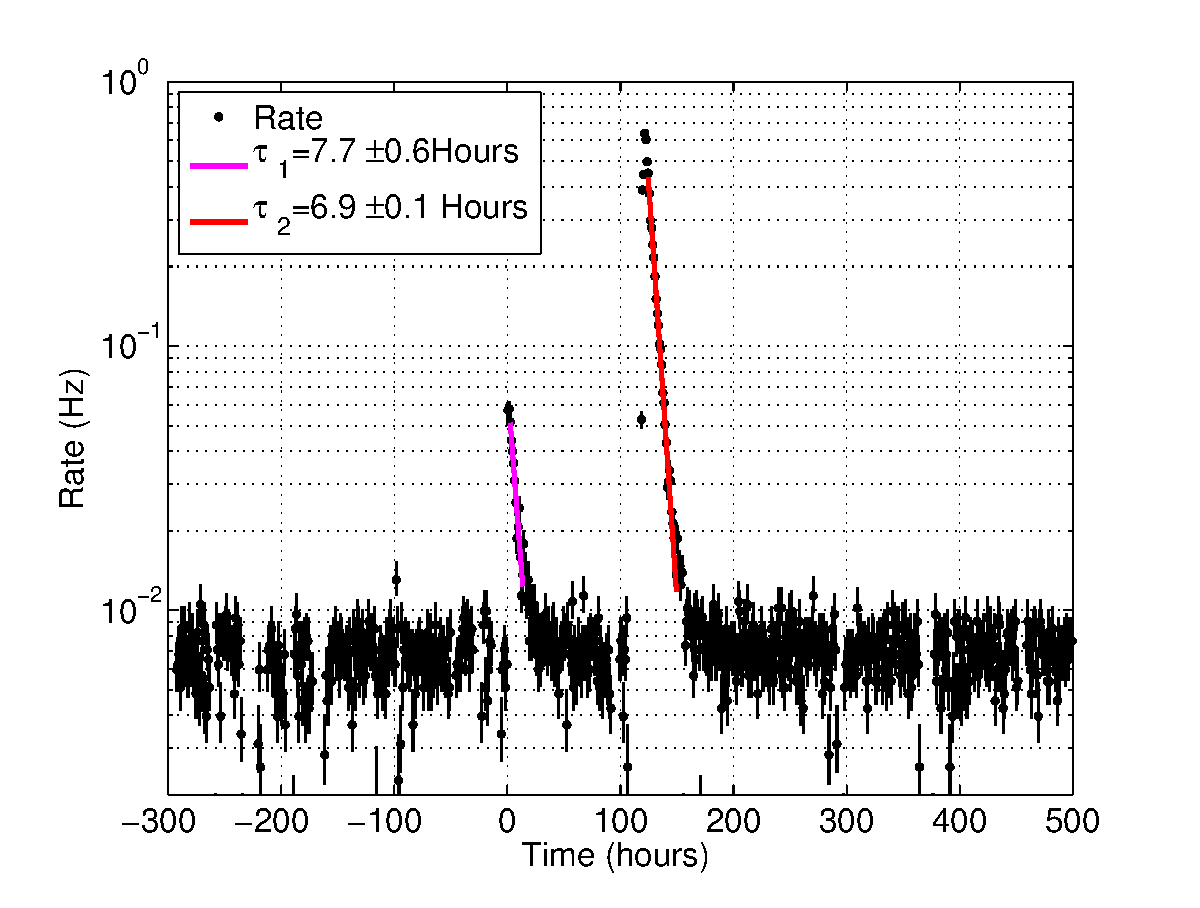
\includegraphics[width=60mm]{Chapter_T/Figures/CH3T_Rate_Nofid_150_Run03_Tritium_Rate}
\caption{ The rate of single scatter events with S1 below 100 PE in the fiducial volume. (100 PE in S1 is about 18.6 $\rm keV_{ee}$, the endpoint to the tritium beta spectrum). The magenta and red curves are fits to the first and second tritium injection's removal rate. The removal rate of tritiated-methane from the liquid is consistent with the natural methane removal rate observed in the gas by the gas analysis system (figure \ref{fig:Removal_Methane}.}
\label{fig:Removal}
\end{figure}
\renewcommand{\baselinestretch}{2}
\small\normalsize



\subsection{Mixing of Tritiated Methane in Liquid Xenon}

Tritium events appear uniformly distributed in the liquid xenon volume several minutes after injecting the tritiated-methane into with the xenon gas circulation path. Figure \ref{fig:Density} shows the $\rm R^2$ vs. Z distribution of tritium events thirty minutes after an injection. The events shown cover the region from the gate to the cathode and radially outward to the edge of the detector. %An additional cut requiring that the event be between $\rm \pm 3 \sigma$ of the ER mean was made to disregard residual alpha events from the walls and cathode, the event rate consisted overwhelmingly of tritium events. The tritiated-methane dispersed uniformly throughout the liquid xenon illuminating all regions on the detector. 
 
 \renewcommand{\baselinestretch}{1}
\small\normalsize
\begin{figure}[h!]\centering
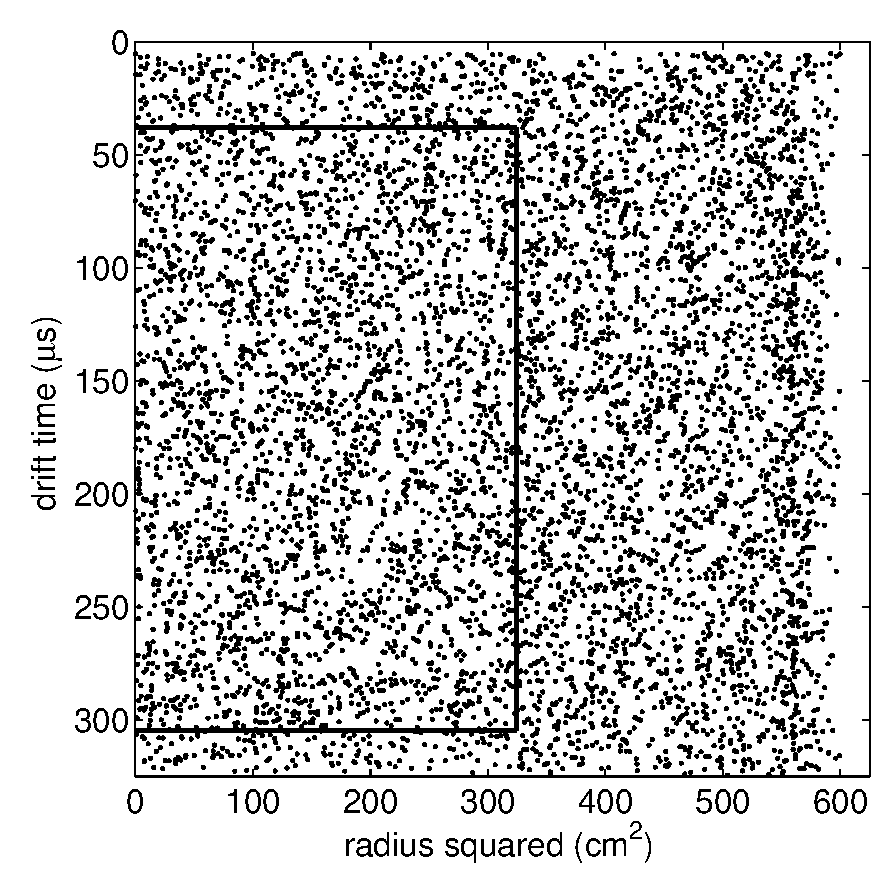
\includegraphics[width=80mm]{Chapter_T/Figures/CH3T_RZ_scatter_lux10_20130812T1546.eps}
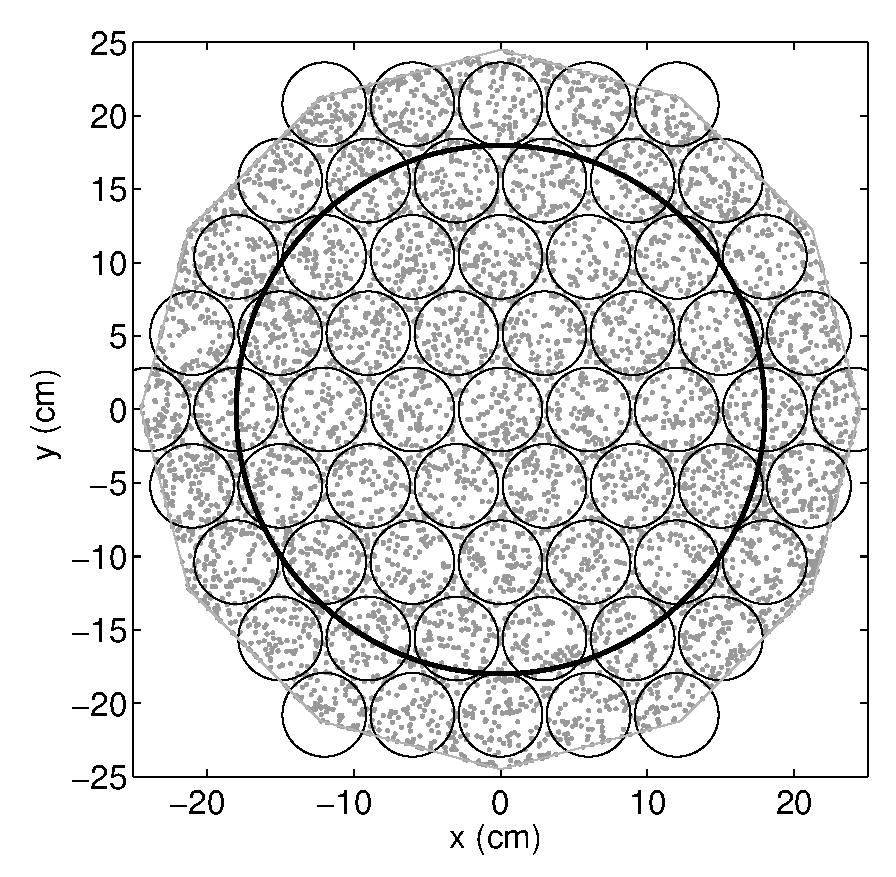
\includegraphics[width=80mm]{Chapter_T/Figures/CH3T_XY_scatter_PMT_lux10_20130812T1546.eps}
%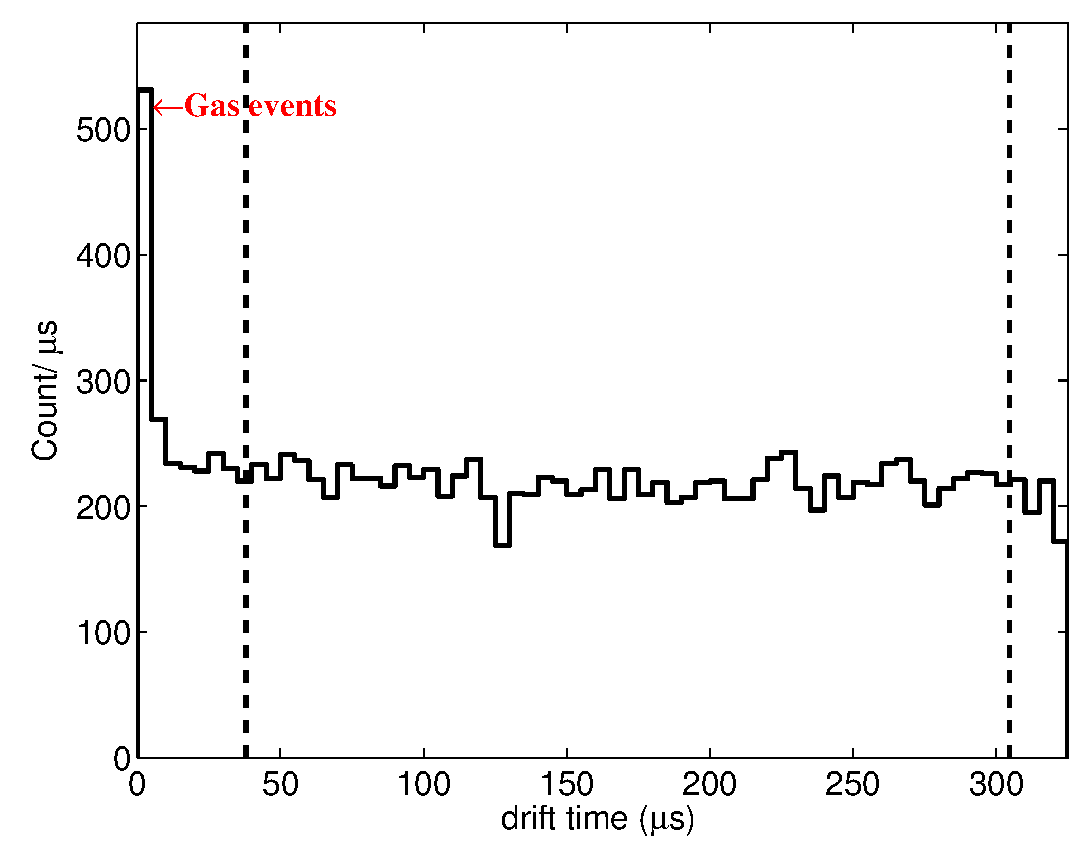
\includegraphics[width=80mm]{Chapter_T/Figures/CH3T_Z_density_lux10_20130812T1546.eps} %> No Need R^2 vs. Z figure contains Z information
\caption{The distribution of tritium events vs. detector radius squared. The solid black line represents the fiducial volume.
 Right: The distribution of tritium events vs. XY in the region between the gate and the cathode. The solid black line represents the fiducial volume and the black circles represent the locations of PMTs (photo multiplier tubes).}
\label{fig:Density}
\end{figure}
\renewcommand{\baselinestretch}{2}
\small\normalsize

\subsection{Definition of the Electronic Recoil Band and the ER Discrimination Factor}

The electronic recoil band in the fiducial volume of the LUX detector was calibrated to unprecedented accuracy using the tritium source. The calibration data was acquired in a 40 hour time window in which less than four out of the 140,000 events in the fiducial are expected to be non-tritium \cite{LUX_BG}.  Nearly every data point (99.997\%) that will be presented in the subsequent figures is the result of a tritium beta decay in the fiducial volume of the LUX detector. 

Figure \ref{fig:Band} shows the tritium calibration data with fits to the mean of the ER band along with the 10-90\% confidence bounds ($\pm 1.28\sigma$), at a drift field of 170 V/cm. Also shown in red is the nuclear recoil (NR) mean measured using a mono-energetic DD neutron generator calibration, described in a future LUX publication.


\renewcommand{\baselinestretch}{1}
\small\normalsize
\begin{figure}[p!]\centering
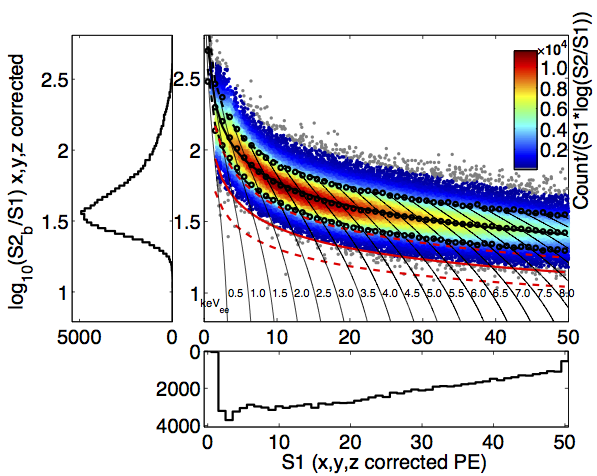
\includegraphics[width=120mm]{Chapter_T/Figures/ER_Band/CH3T_fid_50_rawSpec.png}
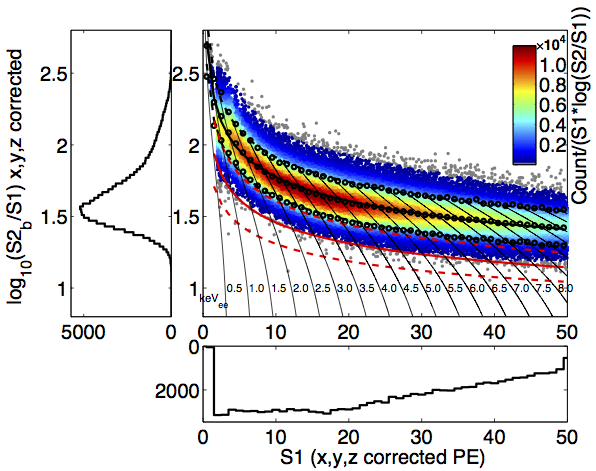
\includegraphics[width=120mm]{Chapter_T/Figures/ER_Band/CH3T_fid_50_proj.png}
\caption{Charge-to-light ratio (log$\rm _{10}(S2_b/S1)$) plotted vs. S1. The energy contours are also shown labeled in $\rm keV_{ee}$. Top, the tritium data uncorrected for spectral shape. Bottom, with the spectral shape correction discussed in section \ref{sec:Smear}. The calibration consists of over 112,000 tritium beta decays between 1 and 50 PE in S1 ($\rm1-10 \, keV_{ee}$), in the fiducial volume of the detector. The black circles represent the ER band mean and 10\% to 90\% bounds, $\rm \pm \,1.28\sigma$. The red solid line is the NR band mean determined using a DD neutron generator calibration. The dashed red lines indicate the 10\% to 90\% bounds of the NR band.}
\label{fig:Band}
\end{figure}
\renewcommand{\baselinestretch}{2}
\small\normalsize
\newpage

The ER band defined by the tritium data shown in figure \ref{fig:Band} has been corrected for spectral shape discussed in section \ref{sec:Smear}. The spectral shape correction recovers the true ER band for a flat energy spectrum. Left uncorrected, the ER band would rise slightly faster in the lowest S1 bins, below 5 PE. 

The ER discrimination factor is defined as the fraction of ER events that do not fall below the mean of the NR band. The ER discrimination can also be thought of as the fraction of ER events that leak below the NR mean, or the leakage fraction. We measure the ER discrimination factor, using the tritium calibration, by counting the number of events that leak below the NR mean. Values of leakage fraction at 50\% NR acceptance per 1 PE bins in S1 are shown in \ref{fig:Leak}. Discrimination and leakage fraction is listed listed at several acceptance fractions in table \ref{table:NR_LeakFrac}. Note, Below 15 PE in S1 the NR acceptance actually becomes greater than 50\% due to the asymmetric shape of the NR band at low energies, which works in our favor \cite{NEST} \cite{NEST_2013}.

\renewcommand{\baselinestretch}{1}
\small\normalsize
\begin{figure}[h!]\centering
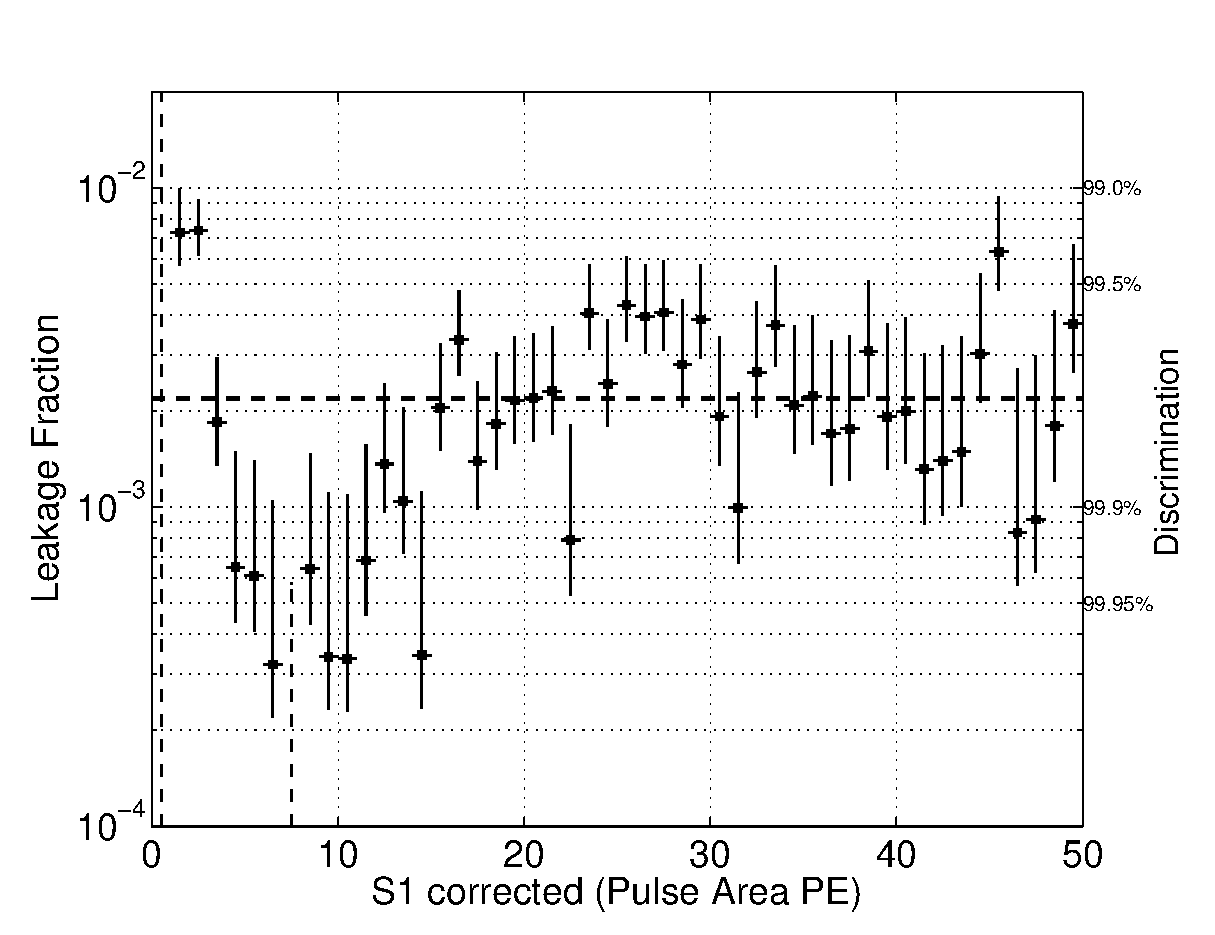
\includegraphics[width=120mm]{Chapter_T/Figures/ER_Band/CH3T_Leakage_fid_50_rawSpec.eps}
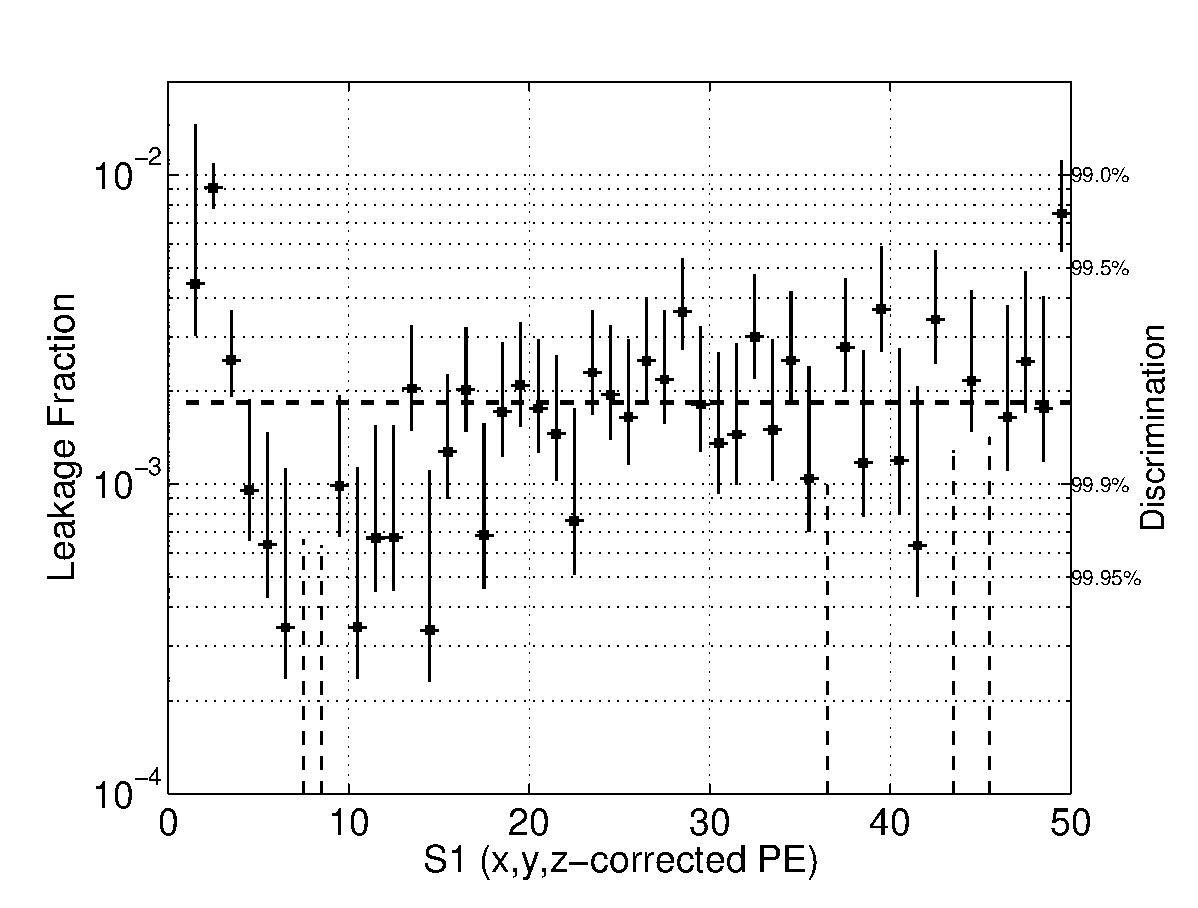
\includegraphics[width=120mm]{Chapter_T/Figures/ER_Band/CH3T_Leakage_fid_50_.eps}
\caption{ER discrimination factor and leakage vs. S1 using over 112,000 tritium beta decays between 1 and 50 PE in S1 ($\rm1-10 \, keV_{ee}$), at 170 V/cm. Top, the tritium data uncorrected for spectral shape. Bottom, with the spectral shape correction discussed in chapter \ref{sec:Smear}. The dashed horizontal lines indicate the mean leakage fraction from 1 to 50 PE.}
\label{fig:Leak}
\end{figure}
\renewcommand{\baselinestretch}{2}
\small\normalsize

%Discrimination Table
\renewcommand{\baselinestretch}{1}
\small\normalsize
\begin{table}[h!]
\begin{center}
\begin{tabular}{|c|c|c|c|c|c|}
\hline
 NR 	& Leakage Fraction 	& Discrimination 		&& Leakage Fraction$^{*}$ 	& Discrimination$^{*}$ \\
 	\%	&$\rm \times 10^{-3}$	&	\%					&&	$\rm \times 10^{-3}$		&	\%				       \\ \hline							
   90  	&	 	52  $\pm$ 0.70  	&	 94.8 $\pm$ 0.07   	&&	49 $\pm$ 0.60   		&	95.1 $\pm$ 0.06 		 \\ \hline
   80   	&		18.8 $\pm$ 0.40	&	 98.1 $\pm$ 0.04   	&&	17.4 $\pm$ 0.40  		&	 98.3 $\pm$ 0.04		\\ \hline
   70  	&	  	8.6  $\pm$ 0.30 	&	 99.1 $\pm$ 0.03   	&&	 7.6 $\pm$ 0.30   		&	99.2 $\pm$ 0.03		\\ \hline
   60  	&	  	4.2 $\pm$ 0.20  	&	 99.58 $\pm$ 0.02  	&&	 3.7 $\pm$ 0.20  		&	 99.63 $\pm$ 0.02		\\ \hline 
   50  	&	  	2.1 $\pm$ 0.14  	&	 99.79 $\pm$ 0.014   	&&	 1.8 $\pm$  0.13  		&	 99.82 $\pm$ 0.013	\\ \hline 
   40  	&	  	0.97  $\pm$ 0.09  	&	 99.90 $\pm$ 0.009  	&&	  0.87 $\pm$ 0.09  	&     99.91 $\pm$ 0.009	\\ \hline
   30  	&	  	0.49 $\pm$ 0.07  	&	 99.95 $\pm$ 0.007  	&&	  0.44 $\pm$ 0.06  	&      99.96 $\pm$ 0.006	\\ \hline
   20  	&	  	0.23 $\pm$ 0.05 	&	 99.977 $\pm$ 0.005  	&&   0.22 $\pm$ 0.04  		&	 99.978 $\pm$ 0.004	\\ \hline
   10   	&		0.08  $\pm$ 0.03	&	 99.992 $\pm$ 0.003	&&	  0.08 $\pm$ 0.03 		&	 99.992 $\pm$ 0.003	\\ \hline
\end{tabular}
\caption{Leakage fraction at various NR acceptance \% over the range of 1-50 PE in S1, using tritium data at 170 V/cm. For the case without spectral shape correction, and with spectral shape correction (columns marked with $^*$). These are conservative estimates assuming Gaussian behavior for NR events about the mean. Below 15 PE in S1 the NR band actually becomes bottom heavy, which works in our favor by increasing NR acceptance \cite{NEST} \cite{NEST_2013}.}
\label{table:NR_LeakFrac}
\end{center}
\end{table}
\renewcommand{\baselinestretch}{2}
\small\normalsize

\newpage

\section{ER Band Gaussianity}
With the high-statistics tritium data set we can test the Gaussianity of the ER band in the WIMP search region. The charge-to-light ratio used to discriminate ER and NR events (plotted as log(S2/S1) in figure \ref{fig:Band}) has been assumed to be Gaussian in past experiments. The largest tritium calibration yielded 112,000 tritium beta decays with only four expected to be non-tritium events \cite{LUX_BG} in the LUX fiducial region. Figure \ref{fig:Gaussianity} shows the same ER band of figure \ref{fig:Band} but with the centroid subtracted, and is plotted with and without the spectral shape correction. We find that below 3 sigma of the ER mean the fluctuations begin to deviate from Gaussian, potentially due to instrumental effects. For example, the probability of finding an ER event 4 sigma below the ER mean is nearly 10 times higher than the probability that would be naively assumed for a purely Gaussian PDF. If not treated properly by data-driven calibrations, such and event could be falsely interpreted as a WIMP event by a profile likelihood analysis.

\renewcommand{\baselinestretch}{1}
\small\normalsize
\begin{figure}[h!]\centering
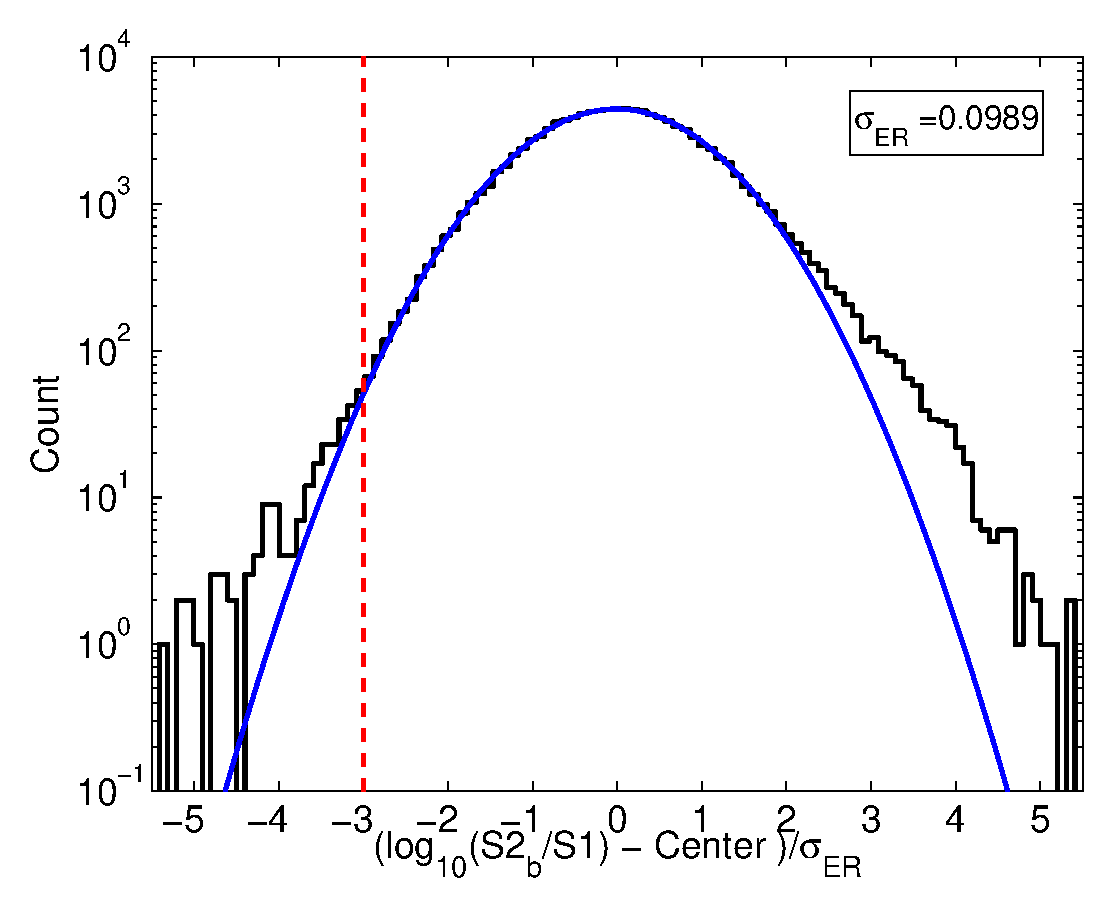
\includegraphics[width=90mm]{Chapter_T/Figures/ER_Band/GaussER_rawSpec.eps}
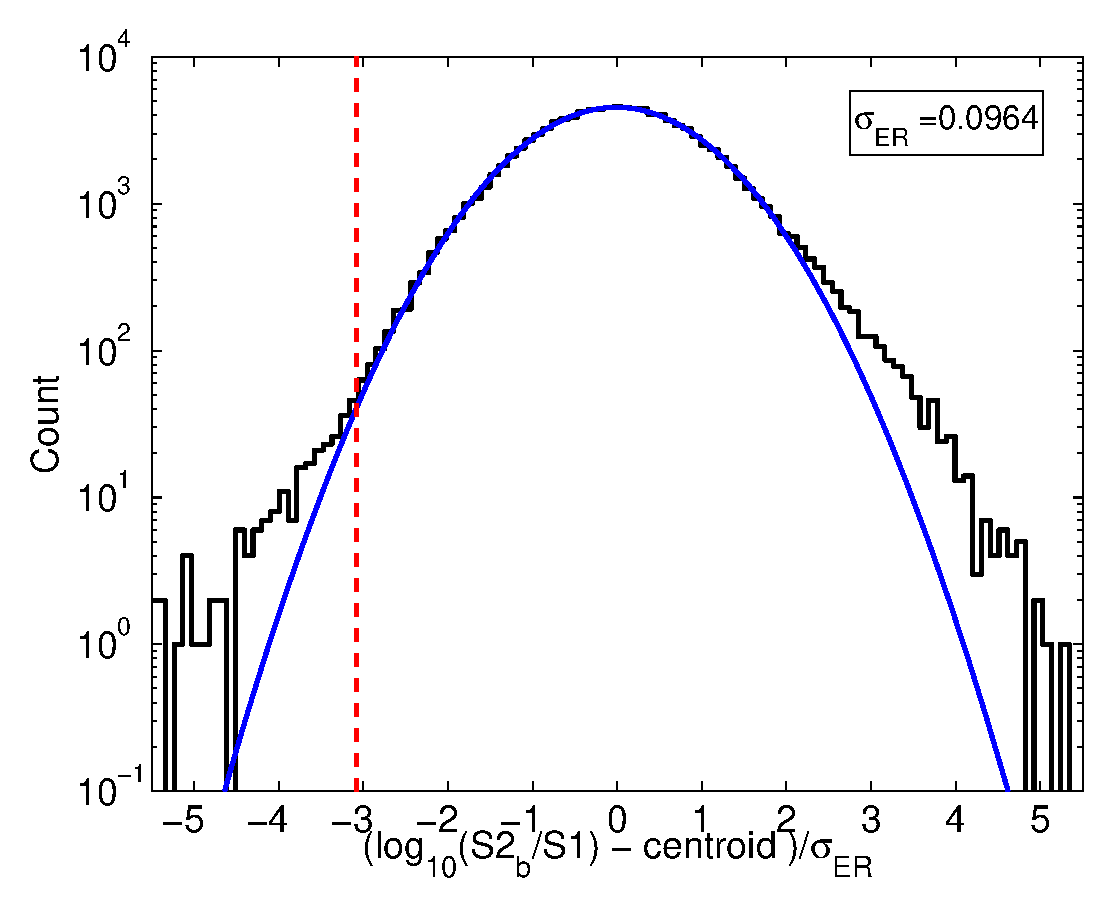
\includegraphics[width=90mm]{Chapter_T/Figures/ER_Band/GaussER.eps}
\caption{ER band Gaussianity from 0-50 PE with the centroid of the ER band subtracted off, using tritium data at 170 V/cm. Top, the tritium data uncorrected for spectral shape. Bottom, with the spectral shape correction discussed in section \ref{sec:Smear}. The dashed vertical red line indicates the mean of the NR band from 1 to 50 PE.}
\label{fig:Gaussianity}
\end{figure}
\renewcommand{\baselinestretch}{2}
\small\normalsize

\newpage

%%%%%%%%%%%%%%%%%%%%%%%%%%%%%%%%%%%%%%%%%%%%%%%%%


\section{S1 Threshold For Golden Events, Using Tritium}

The tritiated-methane calibration source provides beta decays with energies well below the energy threshold of the detector ($\rm 1.5 keV_{ee}$). The energy threshold was measured by comparing to the combined energy to the true tritium spectrum in section \ref{sec:E_Thresh}. The S1 detection threshold for detecting golden events, can be determined in the same manner by taking the ratio of the S1 spectrum observed to expected S1 spectrum. The observed S1 spectrum overlaid with the expected S1 spectrum is shown in figure \ref{fig:S1S2_mapping_2} a). The result for detection efficiency of S1 measured using tritium data at 170 and 100 V/cm is shown in figure \ref{fig:S1_Thresh}, along with the efficiency measured using LED calibrations. The efficiency for detecting S1 signals at 2 PE is found to be 75\%, rising to $>$95\% at 3 PE. The LUX trigger threshold is set by the efficiency for detecting S1 signals.

\renewcommand{\baselinestretch}{1}
\small\normalsize
\begin{figure}[h!]\centering
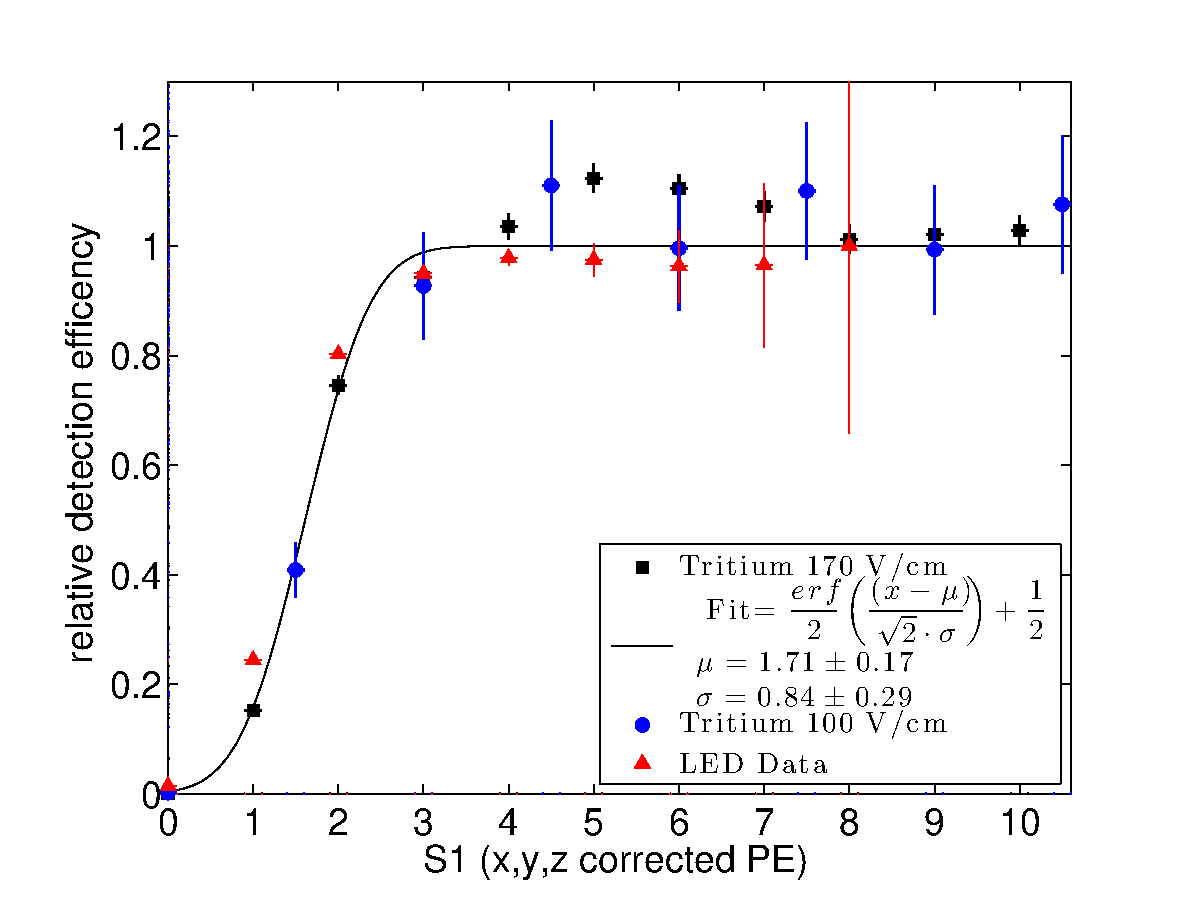
\includegraphics[width=120mm]{Chapter_T/Figures/Threshold/S1_thresh_iter1_led.eps}
\caption{The S1 detection efficiency measured from tritium data at 170 V/cm (black square) and 100 V/cm (blue circle) is plotted along with the best fit to an error function to the higher statistics 170 V/cm data. The red triangles are detection efficiency determined from LED pulsing. }
\label{fig:S1_Thresh}
\end{figure}
\renewcommand{\baselinestretch}{2}
\small\normalsize

\begin{comment}
 \subsection{Absolute Rate}
The absolute efficiency for detecting tritium events can be determined by comparing the number of observed events to the number expected. The initial activity injected was calculated to be $0.84 \pm 0.22 $ Bq, with the largest uncertainty coming from the ratio of $\rm CH_3T/CH_4$ from the tritiated-methane source bottle. The purification time constant was measured to be 6.6 hours. From the initial rate and the purification constant we expect to count a total of $20,200 \pm 4,000 $ events in the LUX detector before applying the S1 threshold. With the S1 threshold we expect  $16,000 \pm 3,100 $ `golden' events. The actual count observed in the liquid xenon volume was 20,000 events, which is in good agreement with the expected value taking into account the uncertainty in the initial activity and the purification model. After making fiducial cut $7,700 \pm  1,500$ events were expected and a total of $9,500 \pm 100$ were observed.

\end{comment}
%%%%%%%%%%%%%%%%%%%%%%%%%%%%%%%%%%%%%%%%%%%%%%%%%%%%%%%%%%



\section{Conclusion}

In this chapter we have described the implementation of a tritiated-methane calibration source for the LUX experiment. The primary application of the source is to characterize the ER band in the WIMP search region, of 1-50 PE (1-10 $\rm keV_{ee}$). This is of great importance, as it gauges the detector's ability to reject background (ER) events from potential WIMP signals (NR). The future LUX WIMP search will not have to rely on the assumption that the ER band can be characterized by a Gaussian PDF.  All previous liquid xenon dark-matter searches have relied upon Compton scatter events to calibrate the ER band and due to lack of statistics have assumed ER band Gaussianity in the WIMP search region. We find that the use of a Guassian PDF, for the LUX detector, fails below 3 sigma of the ER mean as shown in figure \ref{fig:Gaussianity}. The deviation may be arising from instrumental fluctuations or is perhaps a fundamental property of electronic recoils. 

Using the tritium calibration data, a data-driven PDF can be constructed to characterize the distribution of ER events in each S1 bin, greatly improving the systematics of the next WIMP search. Fundamental xenon physics could also be probed with the tritium calibration source as discussed in chapters \ref{Ch:E_Scale_Cal}, \ref{Ch:Flucs} and \ref{Ch:LYQY}. The tritium calibration was used to test the energy scale calibration over the range from 1 to 18 $\rm KeV_{ee}$, and to measure the light yield, charge yield and recombination fluctuations, and the detection thresholds down to 1 $\rm keV_{ee}$. The data taken with the LUX detector will allow for improvements to the NEST modeling at low energies. 


 %The new tritium calibration source provided an unprecedented low energy electronic recoil calibration for the LUX dark matter search \cite{LUX_PRL}.
